\documentclass{exam}
\usepackage[utf8]{inputenc}
\usepackage{lmodern}
\usepackage{microtype}

% \usepackage[parfill]{parskip}
\usepackage[dvipsnames]{xcolor}
\usepackage{amsmath}
\usepackage{amsfonts}
\usepackage{amsthm}
\usepackage{siunitx}
\DeclareSIUnit\year{yr}
\DeclareSIUnit\foot{ft}
\DeclareSIUnit\litre{\liter}

\usepackage{skull}

\usepackage{pgfplots}
\usepgfplotslibrary{polar}
\pgfplotsset{compat=1.11}
\usepgfplotslibrary{statistics}
\usepackage{graphicx}
\usepackage{sidecap}
\sidecaptionvpos{figure}{c}
\usepackage{float}
\usepackage{gensymb}
\usepackage{tkz-euclide}
\usetkzobj{all}
\usepackage{commath}
\usepackage{hyperref}
\usepackage{enumitem}
\usepackage{wasysym}
\usepackage{multicol}
\usepackage{mathtools}
\usepackage{tcolorbox}
\usepackage{tabularx}
\usepackage[version=4]{mhchem}
\usepackage{changepage}
\usepackage{listings}
\lstset{basicstyle=\ttfamily\linespread{0.8}\small}

\renewcommand*{\thefootnote}{\fnsymbol{footnote}}

\newtheorem*{thm}{Theorem}
\newtheorem*{iden}{Identity}
\newtheorem*{lemma}{Lemma}
\newtheorem{obs}{Observation}
\theoremstyle{definition}
\newtheorem*{defn}{Definition}
\newtheorem*{ex}{Example}
\newtheorem{con}{Construction}
\newtheorem*{alg}{Algorithm}

\newtheoremstyle{break}
  {\topsep}{\topsep}%
  {\itshape}{}%
  {\bfseries}{}%
  {\newline}{}%
\theoremstyle{break}
\newtheorem*{bthm}{Theorem}

% russian integral
\usepackage{scalerel}
\DeclareMathOperator*{\rint}{\scalerel*{\rotatebox{17}{$\!\int\!$}}{\int}}

% \DeclareMathOperator*{\rint}{\int}

\pgfplotsset{vasymptote/.style={
    before end axis/.append code={
        \draw[densely dashed] ({rel axis cs:0,0} -| {axis cs:#1,0})
        -- ({rel axis cs:0,1} -| {axis cs:#1,0});
    }
}}

% \pointsinrightmargin
\boxedpoints
\pointname{}

\newcommand{\questioA}{\question[\texttt{\textbf{\color{Cerulean} A}}]}
\newcommand{\questioM}{\question[\texttt{\textbf{\color{PineGreen} M}}]}
\newcommand{\questioE}{\question[\texttt{\textbf{\color{WildStrawberry} E}}]}
\newcommand{\questioS}{\question[\texttt{\textbf{\color{Goldenrod} S}}]}
\newcommand{\questioO}{\question[\texttt{\textbf{\color{BurntOrange} O}}]}

\newcommand{\parA}{\part[\texttt{\textbf{\color{Cerulean} A}}]}
\newcommand{\parM}{\part[\texttt{\textbf{\color{PineGreen} M}}]}
\newcommand{\parE}{\part[\texttt{\textbf{\color{WildStrawberry} E}}]}
\newcommand{\parS}{\part[\texttt{\textbf{\color{Goldenrod} S}}]}
\newcommand{\parO}{\part[\texttt{\textbf{\color{BurntOrange} O}}]}

\newcommand{\subparA}{\subpart[\texttt{\textbf{\color{Cerulean} A}}]}
\newcommand{\subparM}{\subpart[\texttt{\textbf{\color{PineGreen} M}}]}
\newcommand{\subparE}{\subpart[\texttt{\textbf{\color{WildStrawberry} E}}]}
\newcommand{\subparS}{\subpart[\texttt{\textbf{\color{Goldenrod} S}}]}
\newcommand{\subparO}{\subpart[\texttt{\textbf{\color{BurntOrange} O}}]}

\newcommand{\mainHeader}[2]{\section*{NCEA Level 2 Mathematics\\#1. #2}}
\newcommand{\mainHeaderHw}[2]{\section*{NCEA Level 2 Mathematics (Homework)\\#1. #2}}
\newcommand{\seealso}[1]{\begin{center}\emph{See also #1.}\end{center}}
\newcommand{\drills}[1]{\begin{center}\emph{Drill problems: #1.}\end{center}}
\newcommand{\basedon}[1]{\begin{center}\emph{Notes largely based on #1.}\end{center}}

\begin{document}

\mainHeaderIntg{22}{Lengths, Volumes, and Areas}
Recall that the definite integral is simply a way of calculating the area bounded by a curve. We defined
it to be an infinite sum of areas under the curve that individually tended to zero.
\begin{center}
  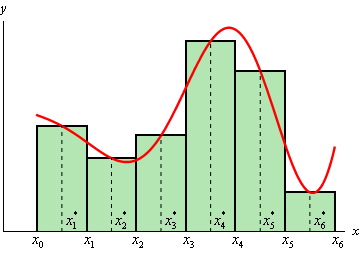
\includegraphics[width=0.4\linewidth]{approx-rectangles}
\end{center}

Today we will investigate finding volumes, curve lengths, and areas of surfaces by integration.

\subsection*{Curve Lengths}
\begin{center}
  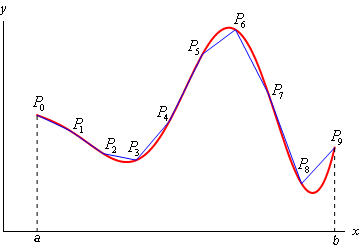
\includegraphics[width=0.4\linewidth]{arclength}
\end{center}
Suppose we have a function $ f $ and we wish to find the length \textit{measured along the curve}
between two points $ a $ and $ b $. Split the interval into pieces of length $ \Delta x $; then the
arc length over each subdivision is approximated by $ \sqrt{\Delta x^2 + (f'(x_i^\ast) \Delta x)^2 } $ where $ x_i $ is
a point inside the subdivisioon. We therefore have the sum over the whole interval $ (a,b) $ (where the total number
of subdivisions is $ n $):
\begin{displaymath}
  \sum_{i = 0}^n \sqrt{\Delta x^2 + (f'(x_i^\ast) \Delta x)^2 } = \sum_{i = 0}^n \sqrt{1 + (f'(x_i^\ast))^2} \Delta x.
\end{displaymath}

But if we let $ n \to \infty $, this is exactly the following integral:
\begin{displaymath}
  R = \rint^b_a \sqrt{1 + (f'(x))^2} \dif{x}.
\end{displaymath}

\begin{ex}
  We wish to find the length along the curve $ y = \ln \cos x $ along the interval $ (0, \pi/3) $. We have the
  following integral (noting that $ y' = -\frac{\sin x}{\cos x} = -\tan x $):
  \begin{align*}
    R = \rint^{\pi/3}_0 \sqrt{1 + \tan^2 x} \dif{x} &= \rint^{\pi/3}_0 \sec x \dif{x}
                                                     = \rint^{\pi/3}_0 \frac{\sec^2 x + \sec x \tan x}{\sec x + \tan x} \dif{x}
                                                    = \rint^{2 + \sqrt{3}}_{1} \frac{1}{u} \dif{u}
                                                     =  \ln(2 + \sqrt{3}) \approx 1.3170.
  \end{align*}
  \textit{The integral of $ \sec $ is tricky; it can also be done by partial fractions (multiply top and bottom of $ 1/\cos x $
          by $ \cos x $ and substitute $ u = \sin x $).}
\end{ex}

\subsection*{Volumes of Revolution}
\begin{center}
  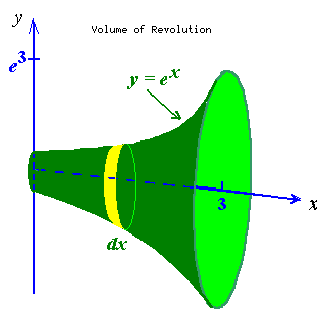
\includegraphics[width=0.4\textwidth]{revs}
\end{center}
We can carry out the same procedure to find a volume of revolution; the volume of each small disc can be approximated
with $ \pi [f(x_i^\ast)]^2 \Delta x $, and so we have
\begin{align*}
  V &= \lim_{n \to \infty} \sum_{i=0}^n \pi [f(x_i^\ast)]^2 \Delta x\\
    &= \rint_a^b \pi [f(x)]^2 \dif{x}.
\end{align*}

\subsection*{Surface Areas of Revolution}
We can model the surface area of revolution of a curve is similarly found by modelling the volume as a disc of
radius $ f(x_i^\ast) $ and length $ \sqrt{1 + (f'(x_i^\ast))^2} \Delta x $:
\begin{align*}
  A &= \lim_{n \to \infty} \sum_{i=0}^n 2\pi f(x_i^\ast) \sqrt{1 + (f'(x_i^\ast))^2} \Delta x\\
    &= \rint_a^b 2\pi f(x) \sqrt{1 + (f'(x))^2} \dif{x}.
\end{align*}

\clearpage
\subsection*{Questions}
\begin{questions}
  \questioM Determine the length of:
    \begin{parts}
      \part $ x = \frac{2}{3} (y-1)^{3/2} $ between $ 1 \leq y \leq 4 $.
      \part $ y = \ln \sec x $ between $ 0 \leq x \leq \frac{\pi}{4} $.
    \end{parts}
  \questioM The arc of the parabola $ y = x^2 $ from $ (1,1) $ to $ (2,4) $ is rotated about the $ y$-axis. Find the area
            of the resulting surface.
  \questioE
    \begin{parts}
      \part Suppose $ f $ is a function of $ x $, and that you know that the graph $ y = f(x) $ is
            a straight line. Furthermore, assume that $ f(0) = 0 $ and $ f(h) = r $ where $ h $ and $ r $
            are constants. Find a formula for $ f $, and draw its graph.
      \part Find a formula for the volume enclosed by rotating the graph $ y = f(x) $ around the $ x$-axis between
            the origin ($ x = 0 $) and $ x = h $. Sketch a diagram showing the volume.
    \end{parts}
  \questioE The cartesian equation for a circle of radius $ r $ is $ y^2 = r^2 - x^2 $. Compute the volume of revolution of the
            circle from $ x = -r $ to $ x = r $, and hence write down the formula for the volume of a sphere of radius $ r $.
  \questioM Find the volume of the solid obtained by rotating the region bounded by the given curves around the $ x$-axis. Sketch
            the region and the solid.
    \begin{parts}
      \part \begin{displaymath}\begin{cases}
              y = 2 - \frac{1}{2}x\\
              y = 0\\
              x = 1\\
              x = 2
            \end{cases}\end{displaymath}
      \part \begin{displaymath}\begin{cases}
              y = x - x^2\\
              y = 0\\
            \end{cases}\end{displaymath}
      \part \begin{displaymath}\begin{cases}
              y = \sqrt{25 - x^2}\\
              y = 0\\
              x = 2\\
              x = 4
            \end{cases}\end{displaymath}
    \end{parts}
  \questioE Find the volume of rotation of the region bounded by $ y = \sin x $ and $ y = \cos x $ around the line $ y = -1 $,
            where $ 0 \leq x \leq \pi/4 $.
  \questioM The ellipse
            \begin{displaymath}
              \frac{x^2}{a^2} + \frac{y^2}{b^2} = 1 \quad\text{where $ a > b $}
            \end{displaymath}
            is rotated around the $ x$-axis to form an ellipsoid. Find the surface area of the ellipsoid.
  \questioM Use Simpson's rule with $ n = 8 $ to estimate the volume of the solid resulting when the region enclosed by the curves
            \begin{displaymath}
            \begin{cases}
             y = \sin^8 x\\
             y = 2x/\pi\\
             x = 0\\
             x = \pi/2
            \end{cases}
            \end{displaymath}
            is revolved around the $ x$-axis.
  \questioS A vase is created by rotating the curve
            \begin{displaymath}
              x = \frac{1}{200} y^3 - \frac{1}{10} y^2 + \frac{3}{2} y + \frac{5}{3}
            \end{displaymath}
            around the $ y$-axis for $ 0 \leq y \leq 20 $ ($ y $ is in centimetres).
    \begin{parts}
      \part Find a function $ V(\alpha) $ for the volume of water in the vase if it is filled up to $ y = \alpha $.
      \part Water flows into the vase at a rate of \SI{10}{\centi\metre\cubed\per\minute}; water flows out at
            a rate directly proportional to the square root of the volume in the vase at time $ t $.
        \begin{subparts}
          \subpart The initial volume of water in the vase at time $ t = 0 $ is \SI{3}{\centi\metre\cubed}. Find the
                   initial height of the water.
          \subpart After three minutes, the volume of water in the vase is \SI{3.6}{\centi\metre\cubed}. Will the vase
                   ever fill completely? If so, how long does it take?
        \end{subparts}
    \end{parts}
  \questioE Use integration to find the volume of a cylinder by taking slices along the cylinder's axis.
  \questioE Use integration to find the volume of a cone by taking slices along the cone's axis.
  \questioS Compute the integral
            \begin{displaymath}
              \rint_{r - t}^t \sqrt{r^2 - x^2} \dif{x}
            \end{displaymath}
            and hence write down an expression for the slice of width $ t $ of a circle of radius $ r $ (figure).
            \begin{center}
              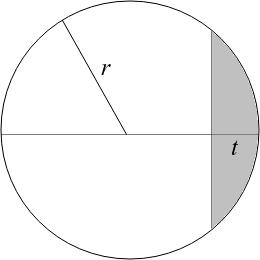
\includegraphics[width=0.3\textwidth]{cslice}
            \end{center}
  \questioS The base of a solid $ S $ is a circle of radius $ r $. Cross-sections perpendicular to the base are squares. What is the volume of $ S $?
  \questioS A cathedral dome is designed with three semicircular supports of radius $ r $ such that each horizontal cross-section is a regular hexagon.
            Show that the volume of the dome is $ r^3\sqrt{3} $.
  \questioE The integral
            \begin{displaymath}
              V = \rint_0^3 2\pi x^5 \dif{x}
            \end{displaymath}
            represents the volume of a solid. Describe the solid.
  \questioO Consider a cylindrical hole of length $ h $ drilled through the centre of a sphere. Find the volume $ V(h) $ of the remaining solid.
            \textit{Hint: you should find that $ V $ is independent of the size of the sphere.}

  \clearpage
  \questioO Two identical right circular cylinders of radius $ r $ have axes that intersect at right angles. Find the volume of
            the intersection region (known as the \textit{Steinmetz solid}). \textit{Hint: an interesting portion of the intersection
            is shown in the figure.\footnote{~Figure from Anton, Early Trans. 10th Ed., p 431.}}
            \begin{center}
              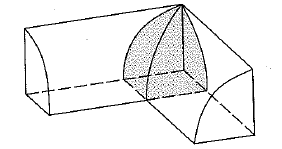
\includegraphics[width=0.3\textwidth]{steinmetz}
            \end{center}
  \questioS Use an integral to estimate the value of the sum
            \begin{displaymath}
              \sum_{n = 0}^{1000000} \sqrt{n}.
            \end{displaymath}
  \questioO A wedge is cut from a right circular cylinder of radius $ r $ by two planes, one perpendicular to the axis of the cylinder
            and one at an angle $ \theta $ with the first (as in the figure\footnote{~Ibid.}). Find the volume of the wedge by slicing perpendicular to
            the $ y$-axis.
            \begin{center}
              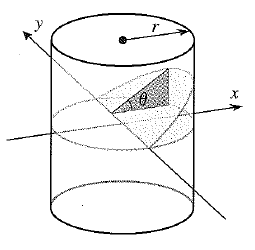
\includegraphics[width=0.3\textwidth]{wedge}
            \end{center}
  \questioS Scholarship 2000: The piriform is the curve defined by the equation $ 16y^2 = x^3(8-x) $ where $ x \geq 0 $.
            Find the volume of revolution obtained by rotating the piriform around the $ x$-axis.
  \questioO Scholarship 2012: Stewie Griffin is a character from the television programme \textit{Family Guy}. His head can be considered
            as a volume of revolution, turning a curve on an axis passing through his ears. Different volumes are obtained, depending on
            the shape of the rotated curve.

            Assuming the head has width $ 2w $ and height $ 2h $, find the \textbf{ratio} of the volume obtained using a parabolic curve
            to the volume obtained using a semi-elliptical curve.
  \questioS Scholarship 2013: Prince Rupert's drops are made by dropping molten glass into cold water. A mathematical model for a drop
            as a volume of revolution uses $ y = \sqrt{\phi (e^{-x} - e^{-2x})} $ for $ x \geq 0 $, where $ \phi $ is the golden
            ratio $ \phi = \frac{1 + \sqrt{5}}{2} $.
    \begin{parts}
      \part Show that the volume of the drop between $ x = 0 $ and $ x = \ln(p) $ is $ V = \frac{\pi \phi}{2} \left( \frac{p - 1}{p} \right)^2 $.
      \part Hence or otherwise, explain why the volume of the drop is never more than some upper limit $ V_L $, no matter how long its tail.
    \end{parts}
  \questioS Scholarship 2015: Find the area of the surface of revolution obtained when the graph of $ f(x) = x^3 + \frac{1}{12x} $,
            from $ x = 1 $ to $ x = 3 $, is revolved \SI{360}{\degree} around the $x$-axis.
\end{questions}
\end{document}
